% Drawing 69/02-12 -- folder 69, batch 02, archive page 34 (PDF page 35).
% Transcription: dans la marge gauche, deux croquis. En haut, un prisme triangulaire : base $u, v$ (et un troisième sommet $w$ caché), face supérieure $u', v', w'$, une diagonale sur la face avant. En dessous, un prisme plus grand, sommets $u, v$ en bas, $u', v', w'$ au milieu, $u'', v'', w''$ en haut, certaines arêtes et diagonales repassées à l'encre plus foncée
% Kind: two prisms in perspective. Method 2 (schematic redraw from the facsimile). Status: partial.
% Notes: Upper: a triangular prism, top u' w' v' (w' at the back, a short stroke down from it towards the hidden w), base u, v, the sides u' u and v' v, and a diagonal stroke rising from u across the front face (it stops halfway, as on the page). Lower: three levels u'' v'' w'' (top), u' v' w' (middle), u v w (bottom); the edges u'' w'', w'' v'', u'' v'', w'' w' (thick), w' u', w' v', u' v', u v, the sides u'' u' u and v'' v' v, w' w, and the diagonals u w (inked over in its middle) and w v' (thick). All vertices are placed once and every stroke runs between them. Still differs from the facsimile: several strokes are doubled or faint on the page and are drawn once; which level a crossing belongs to is a reading; the pencil letters are placed where they stand. Redrawn 2026-11-09 (issue 128): vertices placed once and every edge drawn between them, labels at \small, strike-outs not drawn; to check again.
% Coordinates: 1 unit = 1 mm = 1/100 of the crop width (bbox in page fractions: [0.17, 0.28, 0.37, 0.46]).
% Redrawn by Claude (claude-opus-5-5), issue #73, 2026-11-09; not checked by a human; not compiled (no TeX in the session).
% Rights: reproduces part of the work -- behind RENDER_TRANSCRIPTS, never published by itself.
\documentclass[tikz,border=3pt]{standalone}
\usepackage{amsmath,amssymb}
\usetikzlibrary{patterns,arrows.meta}
\tikzset{pencil/.style={black!45}, struck/.style={black!35}, mark/.style={circle,draw,inner sep=1.3pt}, pt/.style={circle,fill,inner sep=0.9pt}, opt/.style={circle,draw,fill=white,inner sep=1.1pt}}
\begin{document}
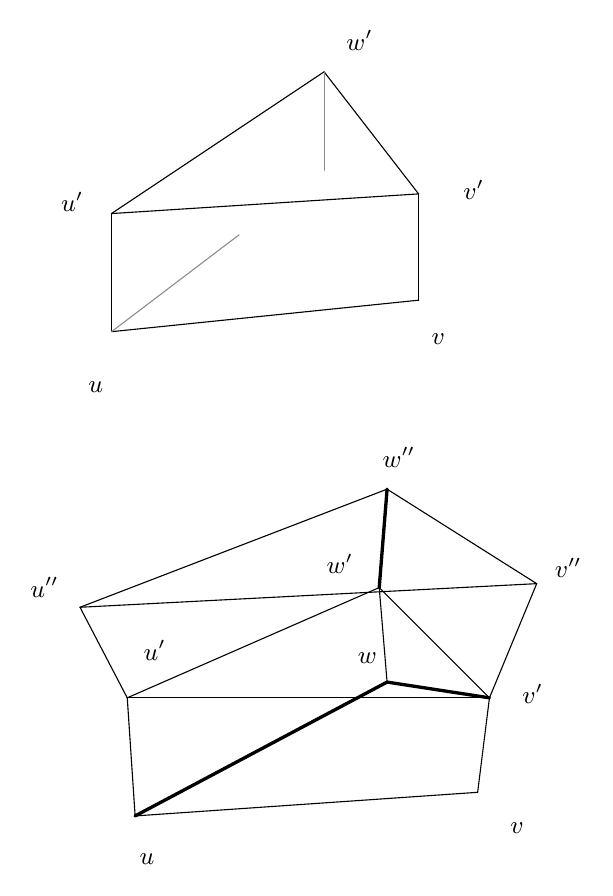
\begin{tikzpicture}[x=1mm,y=1mm,line cap=round,line join=round,font=\scriptsize]
\draw (29,-33) -- (56,-15);
\draw (56,-15) -- (68,-30.5);
\draw (29,-33) -- (68,-30.5);
\draw (29,-33) -- (29,-48);
\draw (68,-30.5) -- (68,-44);
\draw (29,-48) -- (68,-44);
\draw[pencil] (56,-15) -- (56,-27.5);
\draw[pencil] (29,-48) -- (45.2,-35.7);
\node[inner sep=1pt] at (60.5,-11) {\small $w'$};
\node[inner sep=1pt] at (24,-31.5) {\small $u'$};
\node[inner sep=1pt] at (75,-30) {\small $v'$};
\node[inner sep=1pt] at (27,-55) {\small $u$};
\node[inner sep=1pt] at (70.5,-49) {\small $v$};
\draw (25,-83) -- (64,-68);
\draw (64,-68) -- (83,-80);
\draw (25,-83) -- (83,-80);
\draw[very thick] (64,-68) -- (63,-80.5);
\draw (63,-80.5) -- (31,-94.5);
\draw (63,-80.5) -- (77,-94.5);
\draw (31,-94.5) -- (77,-94.5);
\draw (25,-83) -- (31,-94.5) -- (32,-109.5);
\draw (83,-80) -- (77,-94.5) -- (75.5,-106.5);
\draw (32,-109.5) -- (75.5,-106.5);
\draw (63,-80.5) -- (64,-92.5);
\draw[very thick] (32,-109.5) -- (64,-92.5);
\draw[very thick] (64,-92.5) -- (77,-94.5);
\node[inner sep=1pt] at (65.5,-64) {\small $w''$};
\node[inner sep=1pt] at (20.5,-80.5) {\small $u''$};
\node[inner sep=1pt] at (87,-78) {\small $v''$};
\node[inner sep=1pt] at (58,-77.5) {\small $w'$};
\node[inner sep=1pt] at (34.5,-88.5) {\small $u'$};
\node[inner sep=1pt] at (82.5,-94) {\small $v'$};
\node[inner sep=1pt] at (61.5,-89.5) {\small $w$};
\node[inner sep=1pt] at (33.5,-115) {\small $u$};
\node[inner sep=1pt] at (80.5,-111) {\small $v$};
\end{tikzpicture}
\end{document}
